% This is samplepaper.tex, a sample chapter demonstrating the
% LLNCS macro package for Springer Computer Science proceedings;
% Version 2.20 of 2017/10/04
%
\documentclass[runningheads]{llncs}
%
\usepackage{graphicx}
\usepackage{amsfonts}
\usepackage{amsmath}
\usepackage{subcaption}
\usepackage{hyperref}
\usepackage{spverbatim}
% Used for displaying a sample figure. If possible, figure files should
% be included in EPS format.
%
% If you use the hyperref package, please uncomment the following line
% to display URLs in blue roman font according to Springer's eBook style:
% \renewcommand\UrlFont{\color{blue}\rmfamily}

\begin{document}
    %
    \title{Visualization of Aesthetic Anime Objects with The End of Evangelion Vibe}
    %
    \titlerunning{Visualization of Objects with The End of Evangelion Vibe}
    % If the paper title is too long for the running head, you can set
    % an abbreviated paper title here
    %
    \author{Tu Do\inst{1,2}}
    %
    \authorrunning{T. Do}
    % First names are abbreviated in the running head.
    % If there are more than two authors, 'et al.' is used.
    %
    \institute{University of Information Technology, Ho Chi Minh City, Vietnam
    \and
    Vietnam National University, Ho Chi Minh City, Vietnam\\
    \email{18521578@gm.uit.edu.vn}}
    %
    \maketitle              % typeset the header of the contribution
    %
    \begin{abstract}
       Evangelion series can be considered as pieces of media that changed me and somehow helped me through tough times in my life. Even if I change, grow older, and become more mature, I still carry a piece of it years after watching it. Having learned about computer visualization, I get the chance to model myself some of the aesthetic objects from my most beloved anime mentioned above. Specifically, Gendo's glasses, a coffee mug, cigarettes, and ashtray will be illustrated under the scenario of The End of Evangelion. My code is available at: \href{https://github.com/MinhTuDo/IE226}{https://github.com/MinhTuDo/IE226}.

    \keywords{Computer-Generated Imagery \and 
                3DCG \and 
                POV Ray \and CGI}
    \end{abstract}
    
    
    \section{Introduction}
    \label{sect:intro}
    Neon Genesis Evangelion \cite{wikipedia_2021} is a Japanese mecha anime television series produced by Gainax and animated by Tatsunoko, directed by Hideaki Anno, and broadcast on TV Tokyo from October 1995 to March 1996.
    
    Evangelion is set fifteen years after a worldwide cataclysm, particularly in the futuristic fortified city of Tokyo-3. The protagonist is Shinji, a teenage boy who was recruited by his father Gendo to the shadowy organization Nerv to pilot a giant bio-machine mecha named "Evangelion" into combat against beings known as "Angels". The series explores the experiences and emotions of Evangelion pilots and members of Nerv as they try to prevent Angels from causing more cataclysms. In the process, they are called upon to understand the ultimate causes of events and the motives for human action. The series has been described as a deconstruction of the mecha genre and it features archetypal imagery derived from Shinto cosmology as well as Jewish and Christian mystical traditions, including Midrashic tales and Kabbalah. The psychoanalytic accounts of human behavior put forward by Freud and Jung are also prominently featured.
      
    Director Hideaki Anno's depression \cite{myanimelist.net} is what led to the dark themes of Neon Genesis Evangelion. Budgetary problems and parental complaints about content led to the original ending being scrapped and replaced with an extremely limited-animation ending breaking from the main plot. A movie, End of Evangelion, was later made based in part on the original planned ending and in part on Anno's increasing frustration with the otaku fanbase. The series' mix of psychoanalysis, religious symbolism, and genre deconstruction proved extremely influential on mature anime in the late '90s onward. The Japan Media Arts Festival in 2006 ranked it as the most popular anime of all time.
    
    In this section, I will introduce the objects that I will simulate in my project. The reason I chose to simulate these objects is that they are relatively simple. Moreover, they are typical objects with a gloomy, melancholy atmosphere similar to the atmosphere of the anime series that I mentioned. The simulated objects are more or less appearing in the movie scenes, however, I have incorporated some of my own creations.
    
    \subsection{Shinji's Coffee Mug}
        Shinji Holding a Mug \cite{13_2021} is an image based on an image of the character Shinji Ikari from the anime Neon Genesis Evangelion holding a mug.
        
        \begin{figure}[!ht]
            \centering
            
\includegraphics[width=.3\textwidth]{assets/tumblr_mjkfjrIFyZ1s8r2c1o1_400.jpg}
            \caption{Shinji holding a mug \protect\footnotemark}
            \label{fig:shinji}
            
        \end{figure}
        
        \footnotetext{\href{https://knowyourmeme.com/memes/shinji-holding-a-mug/photos}{https://knowyourmeme.com/memes/shinji-holding-a-mug/photos}}
        
        The image is based on a screenshot from the Neon Genesis Evangelion episode; A Human Work, during a scene in which Ikari confronts his guardian, Misato Katsuragi at breakfast time.
        
        \begin{figure}[!htb]
            \centering
            
\includegraphics[width=.5\textwidth]{assets/51l7cbwfvNL._AC_SY450_.jpg}
            \caption{Shinji's Coffee Mug \protect\footnotemark}
            \label{fig:shinji-mug}
        \end{figure}
        
        \footnotetext{\href{https://www.amazon.com/shinji-holding-mug-White-Ceramic/dp/B07JZ1M2CK}{https://www.amazon.com/shinji-holding-mug-White-Ceramic/dp/B07JZ1M2CK}}
        
        The reason this image became popular is that it looks like he's just about fed up with everyone else's nonsense. And thinking that Shinji would ever do something about it is hilarious.
        
    \subsection{Gendo Glasses}
    Gendo's glasses \cite{glasses} are a pair of gray, oval-shaped, full-rimmed glasses with orange-tinted corrective lenses. They are worn by Ikari Gendo in Neon Genesis Evangelion. Figure \ref{fig:glasses} illustrates the glasses appeared in the anime.
    
    \begin{figure}[!htb]
        \centering
        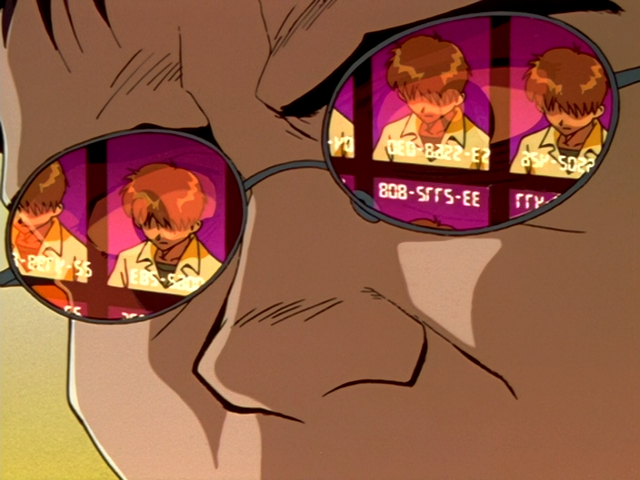
\includegraphics[width=.5\textwidth]{assets/Gendo1.png}
        \caption{Gendou's glasses \protect\footnotemark}
        \label{fig:glasses}
    \end{figure}
    
    \footnotetext{\href{https://anime-glasses.fandom.com/wiki/Gendo\%27s_Glasses_(Neon_Genesis_Evangelion)}{https://anime-glasses.fandom.com/wiki/Gendo}}
    
    \subsection{Cigarettes and Ash Tray}
    Cigarettes and ashtrays have also been featured in Evangelion. They are often seen in anime in the 90s that artistically portray a gloomy and melancholy atmosphere. Figure \ref{fig:cigarette} illustrates the cigarettes and ashtrays that appeared in the anime.
    
    \begin{figure}[!htb]
        \centering
        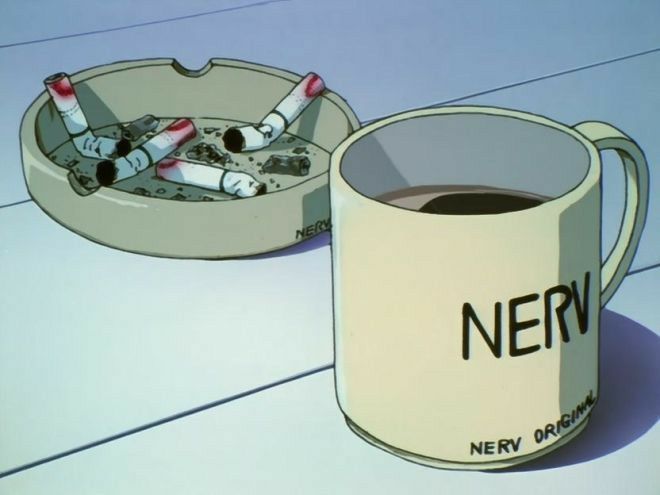
\includegraphics[width=.7\textwidth]{assets/d3820a1d8d6bebd9f0b784e58fc4ac96.jpg}
        \caption{Cigarettes and Ashtrays with Coffee Mug \protect\footnotemark}
        \label{fig:cigarette}
    \end{figure}
    
    \footnotetext{\href{https://www.pinterest.com/pin/756252962418039279/}{https://www.pinterest.com/pin/756252962418039279/}}
    
    \section{POV Ray Background}
    The Persistence of Vision Ray Tracer \cite{pov}, most commonly acronymed as POV-Ray, is a cross-platform ray-tracing program that generates images from a text-based scene description. It was originally based on DKBTrace, written by David Kirk Buck and Aaron A. Collins for Amiga computers.
    
    POV-Ray has matured substantially since it was created. Recent versions of the software include the following features:
    \begin{itemize}
        \item a Turing-complete scene description language (SDL) that supports macros and loops
        \item a library of ready-made scenes, textures, and objects
        \item support for a number of geometric primitives and constructive solid geometry
        \item several kinds of light sources
        \item atmospheric effects such as fog and media (smoke, clouds)
        \item reflections, refractions, and light caustics using photon mapping
        \item surface patterns such as wrinkles, bumps, and ripples, for use in procedural textures and bump mapping
        \item support for textures and rendered output in many image formats, including TGA, PNG, and JPEG, among others
    \end{itemize}
    
    POV-Ray, in addition to standard 3D geometric shapes like tori, spheres, and heightfields, supports mathematically defined primitives such as the isosurface (a finite approximation of an arbitrary function), the polynomial primitive (an infinite object defined by a 15th order or lower polynomial), the Julia fractal (a 3-dimensional slice of a 4-dimensional fractal), the super quadratic ellipsoid (an intermediate between a sphere and a cube), and the parametric primitive (using equations that represent its surface, rather than its interior).

    POV-Ray internally represents objects using their mathematical definitions; all POV-Ray primitive objects can be described by mathematical functions. This is different from many computer programs that include 3D models, which typically use triangle meshes to compose all the objects in a scene.
    
    This fact provides POV-Ray with several advantages and disadvantages over other rendering and modeling systems; POV-Ray primitives are more accurate than their polygonal counterparts: objects that can be described in terms of spheres, planar surfaces, cylinders, tori, and the like, are perfectly smooth and mathematically accurate in POV-Ray renderings, whereas polygonal artifacts may be visible in mesh-based modeling software. POV-Ray primitives are also simpler to define than most of their polygonal counterparts, e.g., in POV-Ray, a sphere is described simply by its center and radius; in a mesh-based environment, a sphere must be described by a multitude of small connected polygons (usually quads or triangles).
    
    On the other hand, script-based primitive modeling is not always a practical method to create certain objects, such as realistic characters or complex man-made artifacts like cars. Those objects can and should be created first in mesh-based modeling applications such as Wings 3D and Blender, and then they can be converted to POV-Ray's own mesh format.
    
    \section{Method}
    In this section, I will present the techniques used in my project to build the objects introduced in section \ref{sect:intro}.
    \subsection{Intersection}
    With two or more shapes it results in a shape which has an area that consists of the area common to all these shapes, the area where the objects are overlapping. \cite{intersection}
    
    \begin{spverbatim}
    intersection{
        box {<-0.5,-0.5,-0.5>,< 0.5,0.5,0.5>
             texture{
               pigment{color rgb<1,0.65,0>}
               finish {phong 0.5}}
            }
        sphere{<0,0,0>,0.66
             texture{
               pigment{color rgb<1,0,0>}
               finish {phong 0.5}}
            }
        rotate<0,-30,0>
        translate<0,0.5,0>
        } // end of intersection ------------
    \end{spverbatim}
    
    \subsection{Difference}
    With the "difference" statement you can subtract from a basic object all subsequent objects from the first one. With this statement it is possible to drill out holes and shape out any kind of notches or beveling you want. This statement is like a milling machine the used milling head has the shape of the objects which are following the base object. The "hole" gets the texture from the subtracted object. \cite{difference}
    
    \begin{spverbatim}
        difference{
            box {<-0.5,0.0,-0.1>,< 0.5,1.0,0.1>
                 texture{ pigment{ color rgb<1,0.65,0>}
                          finish { phong 1.0 }}
                }
            box {<-0.3,0.2,-0.1>,< 0.3,0.8,0.1>
                 texture{ pigment{ color Magenta}
                          finish { phong 1.0 }}
                }
            rotate<0,-30,0> translate<0,0,0>}
    \end{spverbatim}
    
    \subsection{Union and Merge}
    Both commands were used to combine two ore more objects to a new object. The objects may be objects without any physical connections.
    These commands are useful to give different objects the same texture or to transform them together (by scale, rotate, translate or matrix) with only one command. \cite{union}
    
    \begin{spverbatim}
        union{
          sphere{<0,1,0>,0.35}
          cone{<0,0,0>,0.45,<0,1.2,0>,0}
          texture{T_Glass3} interior{I_Glass}
          translate <-0.5, 0, 0>
             }
        merge{ 
          sphere{<0,1,0>,0.35}
          cone{<0,0,0>,0.45,<0,1.2,0>,0}
          texture{T_Glass3} interior{I_Glass}
          translate < 0.5, 0, 0>
             }
    \end{spverbatim}
    
    \subsection{While loop}
    Syntax for while loop in pov-ray \cite{loop} \cite{circular}:
    \begin{spverbatim}
    #declare step = 0;
    #declare steps = 100;
    #while (step <= steps)
      #sphere { step*x, 0.4 pigment {Blue} }
      #declare step = step + 1;
    #end

    \end{spverbatim}
    
    \subsection{Macros}
    The essential custom functions of PoV-Ray. These are blocks of code that make calculations, or make objects, or if used in a series can make many objects with all of them different. Macros are declared like this: \cite{povray}
    \begin{spverbatim}
    macro {Macro_Name}({Macro_Parameters})
      {Macro_Body}
    #end
    \end{spverbatim}
    
    
    \section{Results}
    \subsection{Background}
    To be able to mimic the scene in Evangelion, I had to consult various sources to be able to build a starry sky and be able to easily edit the color of the sky. In addition, seawater effect has also been used to simulate red seawater. However, in order to achieve a similarity to the scene in Evangelion, I used a fog effect with the main color red, and it really worked. Figure \ref{fig:theme} shows that my constructed background is considered similar to the target scene.
    \begin{figure}[!htb]
        \centering
        \begin{tabular}{c c}
            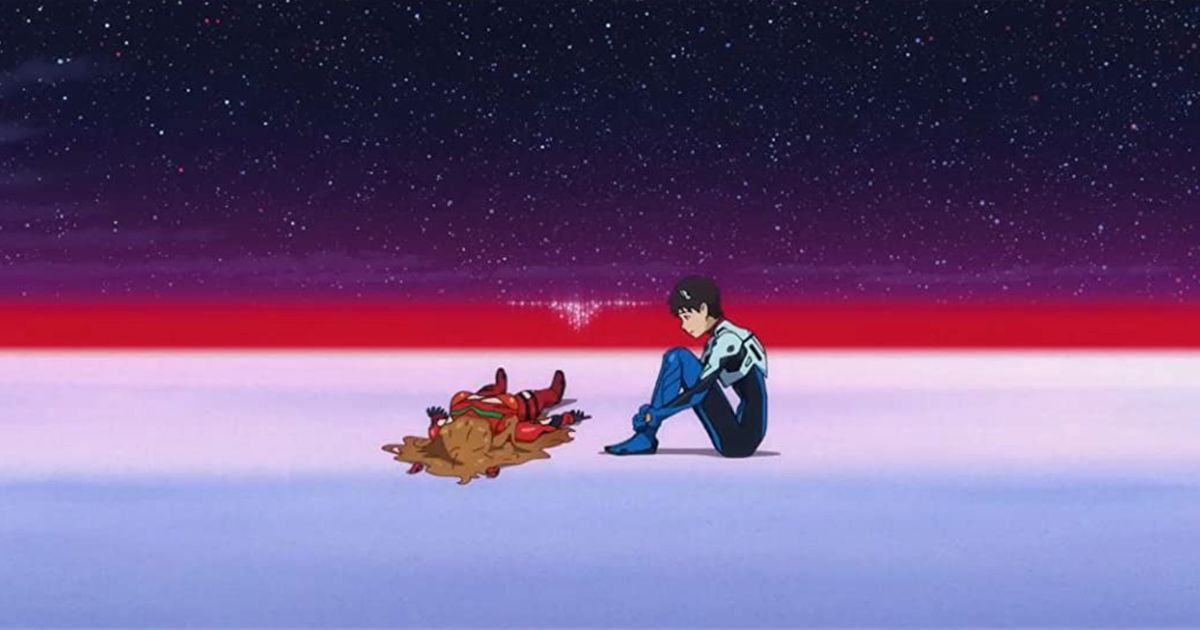
\includegraphics[width=.45\textwidth]{assets/c1ffc823e71d47ba485b61ee39bd40710c-Evangelion.2x.rsocial.w600.jpg} & 
            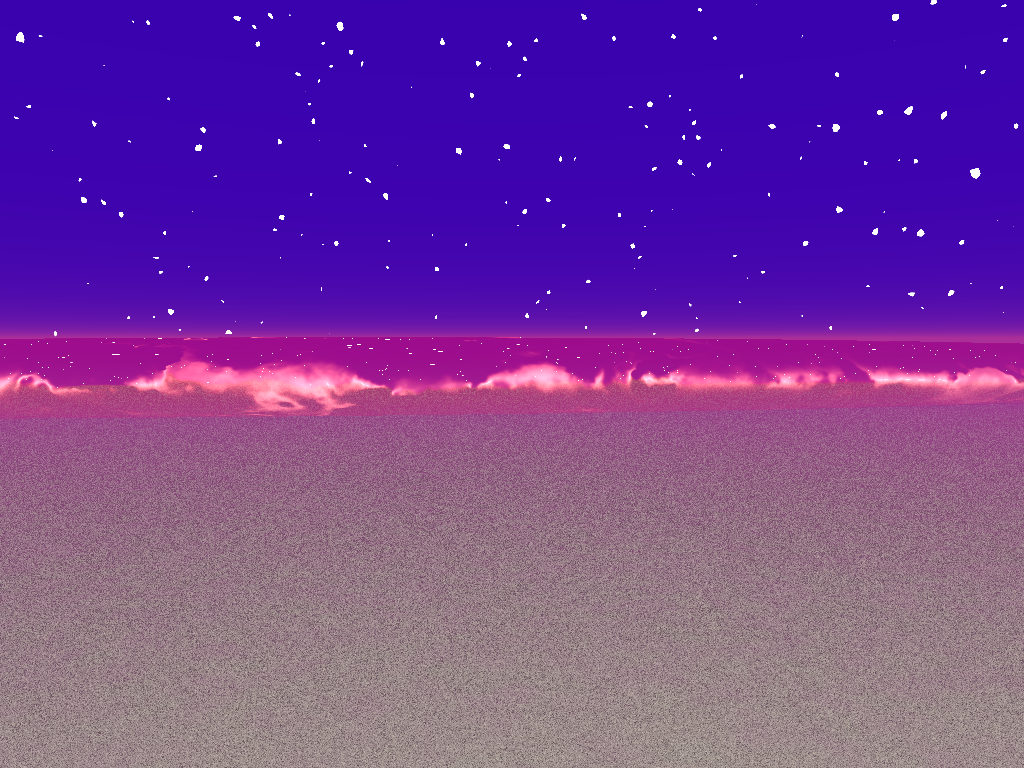
\includegraphics[width=.45\textwidth]{assets/scene.png} \\
        \end{tabular}
        \caption{Comparison of the original scene with reconstructed scene}
        \label{fig:theme}
    \end{figure}
    
    \subsection{Objects}
    Figure \ref{fig:res} illustrates the results obtained when combining the objects with the Evangelion's vibe background. The main drawback is that I haven't been able to attach a single photo to the mug yet. Instead, I could just turn the photo into some kind of pattern so the outside of the cup could be used. Therefore, we can see, the outside of the cup has many duplicate images.
    \begin{figure}[!ht]
        \centering
        \begin{tabular}{c c}
            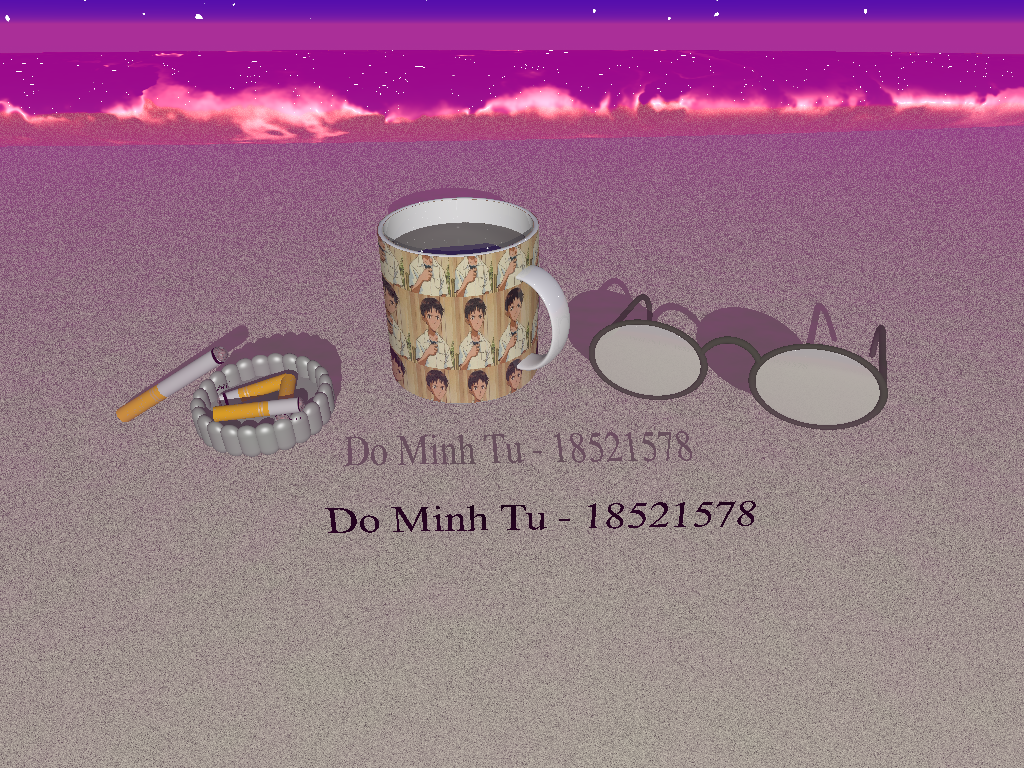
\includegraphics[width=.45\textwidth]{assets/mug.png} & 
            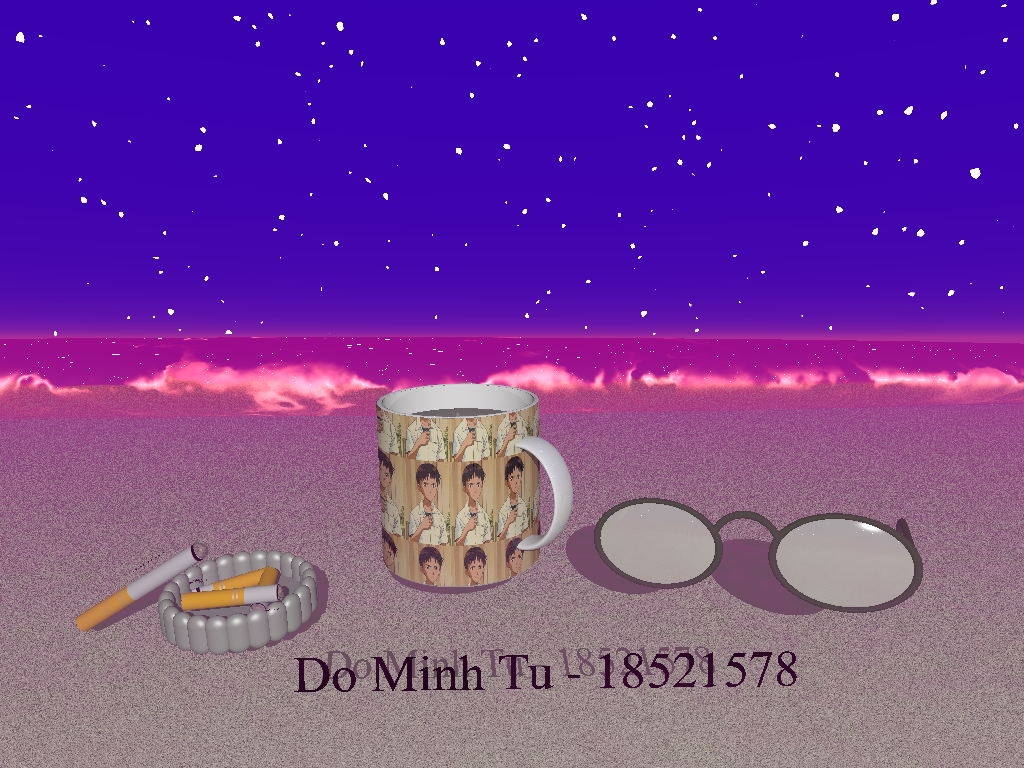
\includegraphics[width=.45\textwidth]{assets/mug1.png} \\
        \end{tabular}
        \caption{Results}
        \label{fig:res}
        \end{figure}   
    
    \section{Conclusions}
    In summary, in this project, I succeeded in building the objects shown in Part A. At the same time, I was also able to build the scene in the style of the anime Evangelion. Overall, I'm very satisfied with the results. However, during the course of the project, I encountered a lot of difficulties in constructing different objects. Specifically, in this project, I built various objects. Therefore, I had to separate each object into different .inc files that could be easily edited. When putting objects in the same context, I had a lot of trouble adjusting the rotation and stretching of the objects together to get good results. In addition, POV Ray does not support real-time compilation, the object building process is very time consuming and trial-and-error. However, with the results achieved, I am completely satisfied with the results I achieved.
    
    \bibliographystyle{splncs04}
    \bibliography{ref}
\end{document}
